\subsection{Tarefa 03 -- Influência da Taxa de Aprendizado}

\begin{comandoquestao}
Objetivo. Investigar como diferentes taxas de aprendizado 
(\texttt{learning\_rate}) afetam a 
convergência e o desempenho da rede neural. Analisaremos como a velocidade e a 
estabilidade do treinamento variam com a alteração dessa taxa.
\end{comandoquestao}

Nessa atividade treinamos uma mesma rede neural com os mesmos dados de testes, 
variando apenas a taxa de aprendizado ($\alpha$) e verificando o seu 
comportamento durante 
o treinamento e a capacidade de previsão da rede. Treinamos as redes para 
$\alpha = 0,001 | 0,01 | 0,05 | 0,1$. A evolução do erro durante o treinamento 
para as redes é mostrada na \cref{tarefa03:tabela:curvas}. As 
capacidades de previsão das redes são mostradas nas 
\cref{tarefa03:0001:predicoes,tarefa03:001:predicoes,tarefa03:005:predicoes,tarefa03:01:predicoes}.

\begin{figure}[tbh]
	\centering
	\caption{Curvas de perda durante treinamento (modificando $\alpha$)}
	\label{tarefa03:tabela:curvas}
	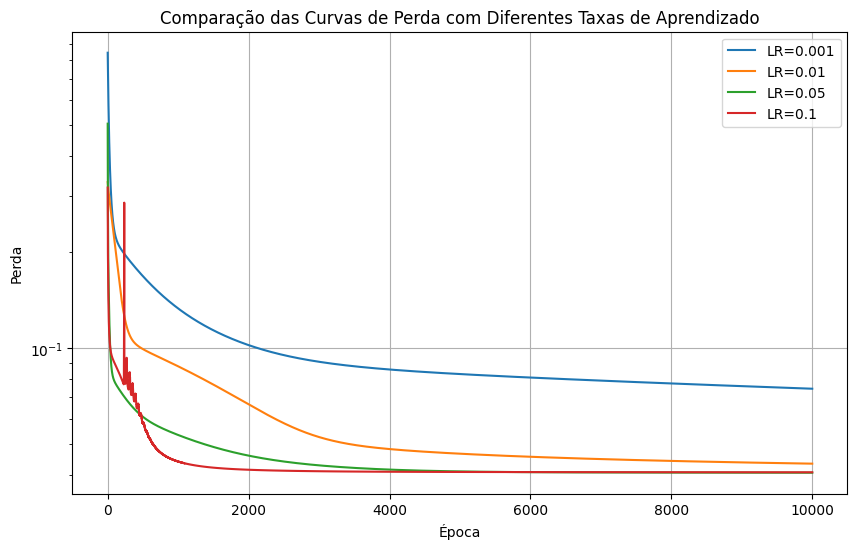
\includegraphics[width=0.7\linewidth]{./0803_imgs/png-241110-180530307-18269409044321663699.png}
\end{figure}


\begin{figure}[htb]
	\centering
	\begin{minipage}{0.45\textwidth}
		\centering
		\caption{$\alpha = 0,001$}\label{tarefa03:0001:predicoes}
		
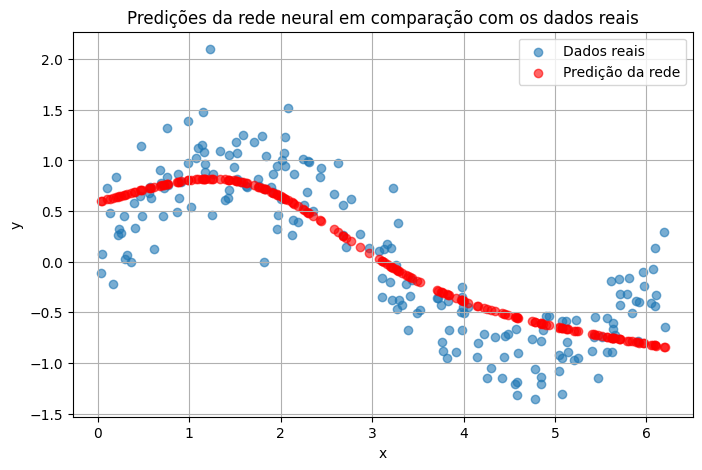
\includegraphics[width=\textwidth]{./0803_imgs/png-241110-175032242-2586281422306343440.png}
		%\legend{Fonte: Gerado peloComando da atividade}
	\end{minipage}
	\hfill
	\begin{minipage}{0.45\textwidth}
		\centering
		\caption{$\alpha = 0,01$}\label{tarefa03:001:predicoes}
		
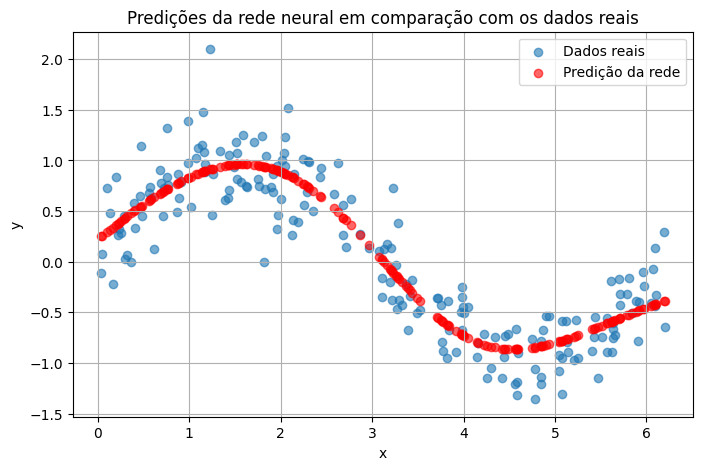
\includegraphics[width=\textwidth]{./0803_imgs/png-241110-175254024-1064294634935646228.png}
		%\legend{Fonte: \citeonline[p. 24]{araujo2012}}
	\end{minipage}
	\vspace{1Ex}
	\begin{minipage}{0.45\textwidth}
		\centering
		\caption{$\alpha = 0,05$}\label{tarefa03:005:predicoes}
		
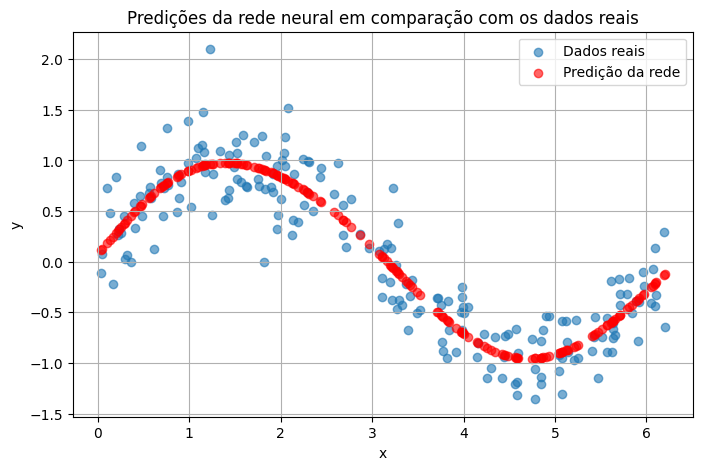
\includegraphics[width=\textwidth]{./0803_imgs/png-241110-175408844-13216912741484706107.png}
%		%\legend{Fonte: \citeonline[p. 24]{araujo2012}}
	\end{minipage}
	\hfill
	\begin{minipage}{0.45\textwidth}
		\centering
		\caption{$\alpha = 0,1$}\label{tarefa03:01:predicoes}
		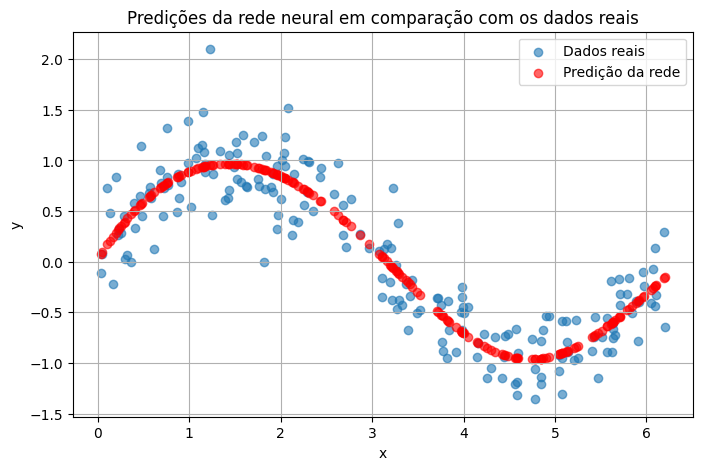
\includegraphics[width=\textwidth]{./0803_imgs/png-241110-175801588-11785230830217735738.png}
		%\legend{Fonte: \citeonline[p. 24]{araujo2012}}
	\end{minipage}
\end{figure}

Ao analisar os resultados com uma taxa de aprendizagem de 0,001, observa-se que 
a convergência é significativamente mais lenta. O modelo parece ficar longe dos 
outros em termos de desempenho. Isso sugere que o modelo pode ter caído em um 
mínimo local, ou que, são necessárias muito mais épocas de treinamento para 
atingir a convergência.

Por outro lado, uma taxa de aprendizagem de 0,05 parece ser um bom equilíbrio. 
Oferece uma convergência mais suave e estável, evitando oscilações extremas, e 
resulta em um bom erro de teste no final do treinamento. Este $\alpha$ pode ser 
uma escolha ideal, pois encontra um compromisso entre a velocidade de 
convergência e a precisão do modelo.

Quando a taxa de aprendizagem é aumentada para 0,1, o gráfico da curva de 
aprendizado parece mais ruidoso e volátil. Isso indica que o modelo pode estar 
enfrentando dificuldades 
para encontrar o mínimo do gradiente nas primeiras épocas do treinamento. Taxas 
de aprendizagem mais altas podem fazer com que o modelo pule o mínimo global e 
resultem em um comportamento mais caótico durante o processo de otimização.

Em resumo, a escolha da taxa de aprendizagem é crucial para o treinamento de 
modelos de aprendizado de máquina. Uma taxa de aprendizagem muito baixa pode 
resultar em convergência lenta, enquanto uma taxa de aprendizagem muito alta 
pode levar a um comportamento instável. Uma taxa de aprendizagem de 0,05 parece 
ser uma escolha adequada para este cenário específico, proporcionando uma 
convergência suave e um bom desempenho final.

